\section*{Lectura 8: Espacios Contractibles y Convexidad.}

\begin{definition}
    Un subconjunto $X$ de $\R^n$ se llama \textbf{convexo} s\'i para todo puntos
    $x,y \in X$, la recta trazada entre $x$ y  $y$ esta contenido en  $X$. Es
    decir, que para todo  $t \in [0,1]$, $(1-t)x+ty \in X$.
\end{definition}

\begin{figure}[h]
    \centering
    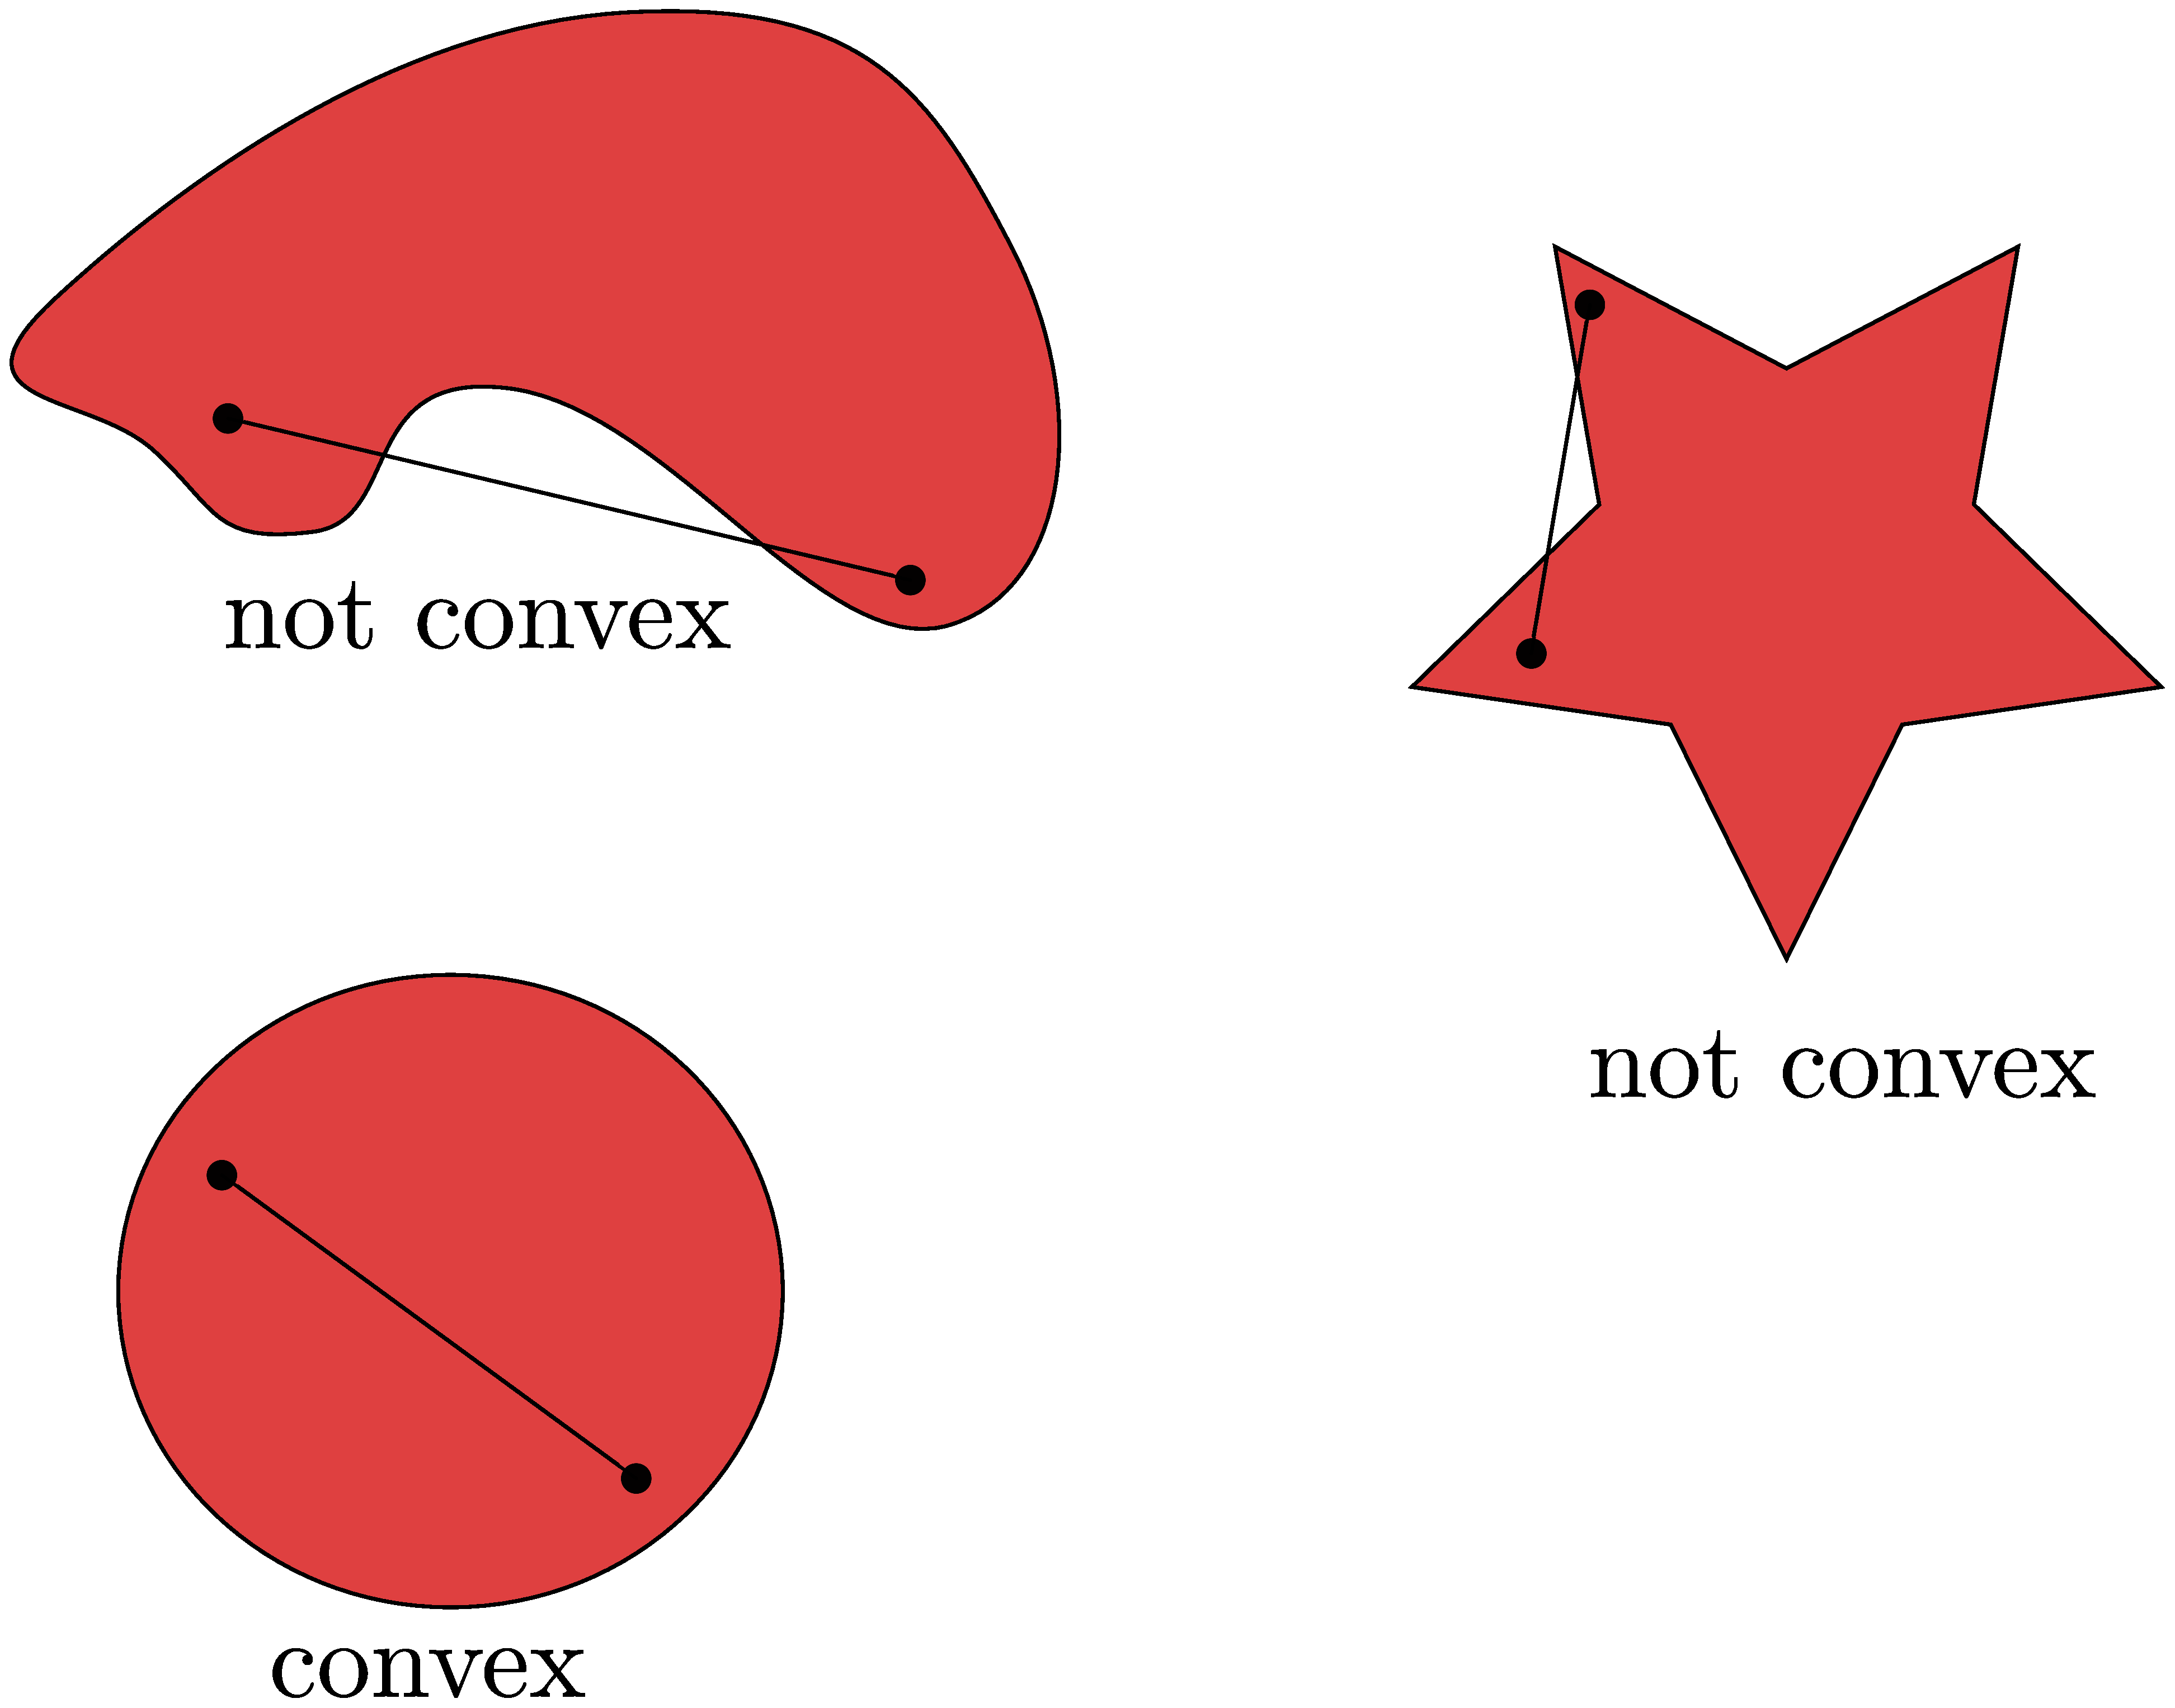
\includegraphics[scale=0.1]{Figures/convex.eps}
    \caption{Espacios convexos y no convexos en $\R^n$. Nota que las estrellas
    no son convexos, pero el disco si es convexo.}
    \label{fig_18}
\end{figure}

\begin{definition}
    Llamamos a un espacio topologico $X$  \textbf{contractible} s\'i la
    identidad en $1_X$ es homotopicamente nula.
\end{definition}

\begin{lemma}\label{lemma_8.13}
    Espacios convexos son contractibles.
\end{lemma}

\begin{example}\label{}
    \begin{enumerate}
        \item[(1)] El disco $D^n$ es contracible como es convexo, pero la esfera
            $S^{n-1}$ no es contractible como $1_{S^{n-1}}$ no puede ser
            homotopicamente nula.

        \item[(2)] EL hemisferio norte de $S^{n-1}$, $H^+=\{x \in S^{n-1} :
            x_{n-1}=0\}$ es contractible, pero no convexo. S\'i una considere
            los geodesicos sobre $H^+$ como las rectas, entonces resulta que
            s\'i  $H^+$ es convexo.
    \end{enumerate}
\end{example}

\begin{definition}
    Sea $X$ un espacio topologico y $X'$ una partici\'on de $X$ en conjuntos
    disjuntos  $X_\alpha$. Definimos la  \textbf{aplicaci\'on canonica} de $X$
    sobre  $X'$ de ser la mapa $q:X \xrightarrow{} X'$ tal que $q:x \xrightarrow{}
    X_\alpha$ s\'i $x \in X_\alpha$.
\end{definition}

\begin{definition}
    Sea $X$ un espacio topologico,  $X'$ una partici\'on de  $X$, y  $q:X
    \xrightarrow{} X'$ la aplicaci\'on canonica de $X$ sobre $X'$. Definimos el
    \textbf{topologia cociente} de $X'$ de ser la colecci\'on
    \begin{equation*}
        \Tc=\{U \subseteq X' : \inv{q}(U) \text{ es abierto en } X\}
    \end{equation*}
    Llamamos a $X'$ bajo este topologia el  \textbf{espacio cociente} de $X$.
\end{definition}

\begin{lemma}\label{lemma_8.14}
    S\'i $X$ es un espacio topologico, y  $X'$ es su espacio cociente, entonces
    la aplicaci\'on canonica de  $X$ sobre  $X'$ es continua. Es decir que $q
    \in \Hom{(X,X')}$ en la categoria $\Top$.
\end{lemma}

\begin{definition}
    Sea $X$ un espacio topologico y  $A \subseteq A$. Defina
    $\faktor{X}{A}=\{A\} \cup \{y \in X : y \notin A\}$. Se llama a
    $\faktor{X}{A}$ bajo el topolog\'ia cociente el \textbf{espacio cociente} de
    $X$  \textbf{colapsada} por $A$. Decimos que $A$ \textbf{colapsa} a un punto
    bajo la topologia cociente.
\end{definition}

\begin{example}\label{}
    \begin{enumerate}
        \item[(1)] S\'i $X=[0,1]$ y $A=\{0,1\}$, entonces el espacio cociente
            $\faktor{X}{A} \simeq S^1$ es homeomorfo al circulo. Se mostra de
            como se puede llegar de $[0,1]$ hasta $S^1$ en el figura \ref{fig_19}.

        \begin{figure}[h]
            \centering
            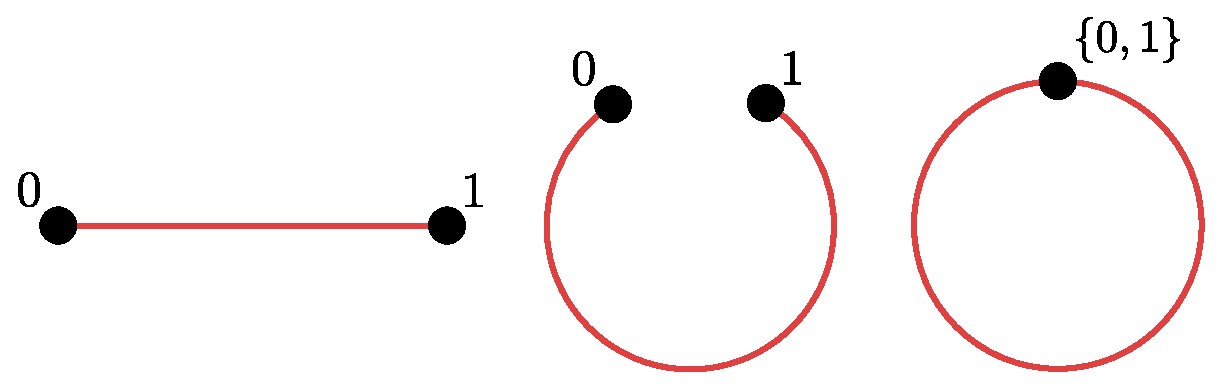
\includegraphics[scale=0.5]{Figures/interval_to_circle.eps}
            \caption{Se puede pensar en la aplicaci\'on canonica de
                $\faktor{[0,1]}{\{0,1\}}$ de coger el intervalo $[0,1]$ y
            deformandolo hasta que pegas el punto $0$ con el punto $1$. El espacio
            resultante es $S^1$.}
            \label{fig_19}
        \end{figure}
        \item[(2)] $\faktor{D^n}{\partial{D^n}}=S^{n-1}$, que no es
            contractible.

        \item[(3)] Sean $h:X \xrightarrow{} Y$ una mapa. Defina la relacion
            $\ker{h}$ dado por $x \ker{h} x'$ s\'i y solo s\'i $h(x)=h(x')x'$.
            Entonces $\faktor{X}{\kewr{h}}=\{\phi([x]), x \in X\}$, donde
            $\phi([x])=h(x)$ forma una topologia bajo la cociente.

            Ahora sea $\phi:\faktor{X}{\ker{h}} \xrightarrow{} Y$ 1--1. Se hace
            la siguiente diagrama commutativa:
            \[\begin{tikzcd}
                X &&& Y \\
                \\
                \\
                {\faktor{X}{ker{h}}}
                \arrow["h", from=1-1, to=1-4]
                \arrow["q"', from=1-1, to=4-1]
                \arrow["\phi"', from=4-1, to=1-4]
            \end{tikzcd}\]

            note que $h$ es continua s\'i y solo s\'i  $\phi$ es continua, mas
            a\'un, s\'i  $h$ lleva a $X$ sobre  $Y$, entonces $\phi$ es un
            homeomorfismo.
    \end{enumerate}
\end{example}

\begin{definition}
    Sean $X$ y  $Y$ espacios topologicos. Una mapa continua de $f:X
    \xrightarrow{} Y$ de $X$ sobre  $Y$ se llama una  \textbf{identificaci\'on}
    si para todo $U$ abierto en  $Y$, $\inv{f}(U)$ esta abierto en $X$.
\end{definition}

\begin{example}\label{}
    \begin{enumerate}
        \item[(1)] S\'i $f: X \xrightarrow{} Y$ es continua de $X$ sobre  $Y$, y
            abieerto o cerrado  (Es decir $U$ abierto o cerrado en  $X$ implica
             $f(U)$ abierto o cerrado en $Y$), entonces $f$ es una
             identifaci\'on. Nota, que  s\'i $U$ esta abierto en  $Y$, entonces
             por continuidad  $\inv{f}(U)$ es abierto en $X$; adem\'as, por ser
             sobre,  $U=f(\inv{f}(U))$ que esta abierto en $Y$. De igaul manera
             se produce lo mismo para cerrados, pero usnado complementos.

         \item[(2)]  Unas identificaci\'ones son la relaci\'on $\ker{h}$ y la
             aplicac\'on canonica.
    \end{enumerate}
\end{example}

\begin{definition}
    Sean $X$, y  $Y$ espacios topologicos, y  $f:X \xrightarrow{} Y$ una
    identificaci\'on. Una mapa $s:X \xrightarrow{} Y$ se llama una
    \textbf{secci\'on} s\'i $f \circ s=1_Y$.
\end{definition}

\begin{definition}
    Sea $f:X \xrightarrow{} Y$ una mapa de un espacio topologico $X$ hacia un
    espacio topologico  $Y$. S\'i $y \in Y$, llamamos  $\inv{f}(y)$ la
    \textbf{fibra} de $f$ sobre  $y$.
\end{definition}

\begin{example}\label{}
    Las fibras de la aplicacion canonica $q$ son los clases de equivalencias
    $[x] \in \faktor{X}{\ker{h}}$, para una mapa $h:X \xrightarrow{} Y$.
\end{example}

\begin{theorem}\label{thm_8.15}
    Sea $f:X \xrightarrow{} Y$ continua de espacios topologicos $X$ sobre  $Y$.
    Entonces, $f$ es una identificaci\'on s\i y solo s\'i para todo espcaio
    topologico $Z$, y un mapa $g: Y \xrightarrow{} Z$, tenemos que $g$ es
    continua s\'i y solo \s'i  $g \circ f$ es continua.
    \[\begin{tikzcd}
        X &&& Y \\
        \\
        Z
        \arrow["f", from=1-1, to=1-4]
        \arrow["g", from=1-4, to=3-1]
        \arrow["{g \circ f}"', from=1-1, to=3-1]
    \end{tikzcd}\]
\end{theorem}
\begin{proof}
    Suponga que $f$ es una identifiacion. Sea  $Z$ un espacio topologico y $g:Y
    \xrightarrow{} Z$. S\'i $g$ es continua, entonces  $g \circ f$ es continua
    por composiciones. Ahora, por otro lado, si  $g \circ f$ es continua,
    entonces dado  $V$ abierto en  $Z$, tenemos que  $\inv{f}(\inv{g}(V))$ es
    abierto en $X$. Como $f$ es sobre, esto hace que  $\inv{g}(V)$ sea abierto
    en $Y$.

    Ahora considere el espacio  $Z$, junto al mapa  $g:Y \xrightarrow{} Z$ tal
    que $g$ es continua s\'i y solo s\'i  $g \circ f$ es continua. Sea  $f$
    continua de  $X$ sobre  $Y$, y sea  $Z=\faktor{X}{\ker{f}}$. Considera la
    aplicaci\'on canonica y la mapa $\phi([x])=f(x)$, donde $\phi$ es 1--1.
    \[\begin{tikzcd}
        X &&& Y \\
        \\
        {\faktor{X}{\ker{f}}}
        \arrow["f", from=1-1, to=1-4]
        \arrow["{\phi^{-1}}"', from=3-1, to=1-4]
        \arrow["q"', from=1-1, to=3-1]
    \end{tikzcd}\]
    La diagrama arriba es commutativa, as\'i que $f=\inv{\phi} \circ q$. As\'i
    que $\phi \circ f=q$, hacinedo  $q$ una identificacion. Entonces, sea
    $g=\inv{\phi}$. Tenemos que $g \circ f$ es continua, como  $g \circ f=q$,
    as\'i que por hipotesis,  $g=\inv{\phi}$ tiene que ser continua. Como $q$
    tambien es una identificacion, esto hace que  $\phi$ sea continua, as\'i que
     $\phi$ es un homeomorfismo. Mas a\'un,  $f=\inv{\phi} \circ q$, as\'i que
     $\inv{f}(U)=\inv{(\inv{\phi} \circ q)}(U)=\inv{q}\phi(U)$. Como $q$ es una
     identificaci\'on,  $\phi(U)$ es abierto, esto hace que $\inv{f}(U)$ sea
     abierto. Es decir, $f$ es una identificaion.
\end{proof}
\begin{corollary}
    Si $f$ es una identificacion, y  $h:X \xrightarrow{} Y$ continua, y
    constante en casda fibra de $f$, entonces  $h \circ \inv{f}:Y \xrightarrow{}
    Z$ es continua.
\end{corollary}
\begin{corollary}
    S\'i $h:X \xrightarrow{} Z$ es una identificaci\'on, entonces la
    aplicaci\'on $\phi:\faktor{X}{\ker{h}} \xrightarrow{} Z$ definida por
    $\phi([x])=h(x)$ es un homeomorfismo.
\end{corollary}

\begin{definition}
    Sea $X$ un espacio topologico. Defina una relacion de equivalencia sobre $X
    \times I$ dado por $(x,t) \sim (x',t')$ s\'i y solo s\'i $t=t'=1$. Denota la
    clase de equivalencia de $(x,t)$ $[x,t]$. Entonces llamamos el espacio
    cociente $\faktor{X \times I}{\sim}$ el \textbf{cono} sobre $X$, denotado
    por  $CX$.
\end{definition}

\begin{figure}[h]
    \centering
    \includegraphics[scale=0.1]{Figures/cono_x.eps}
    \caption{El cono $CX$ sobre $X$, con vertice  $[x,1]$.}
    \label{fig_20}
\end{figure}

\begin{theorem}\label{thm_8.16}
    Para todo espacio topologico $X$, el cono,  $CX$ es contractible.
\end{theorem}
\begin{proof}
    Defina la mapa $F:CX \times I \xrightarrow{} CX$ por $[x,1]$.
\end{proof}

\begin{theorem}\label{thm_8.17}
    El espacio topologico $X$ tiene el mismo tipo de homotopia que un punto s\'i
    y solo s\'i  $X$ es contractible.
\end{theorem}
\begin{proof}
    Sea $\{a\}$ y suponga que $X \simeq \{a\}$. Entonces existen una mapas $f:X
    \xrightarrow{} \{a\}$ y $g:\{a\} \xrightarrow{} X$ con $g \circ f=1_X$ y  $f
    \circ g = 1_{\{a\}}$. Pero vemos que $g \circ f(x)=g(f(x))=g(a)=x_0$ para
    alg\'un $x_0 \in X$, as\'i que $1_X \simeq c_{x_0}$.

    Por otro lado, s\'i $1_X \simeq c_{x_0}$ para alg\'un $x_0 \in X$, definia
    las mapas $f:X \xrightarrow{} \{x_0\}$ y $g:\{x_0\} \xrightarrow{} X$ dados por
    $x \xrightarrow{f} x_0$ y $x_0 \xrightarrow{g} x_0$. Entonces, $f \circ
    g=1_{x_0}$y $g \circ f=1_X$.
\end{proof}
\begin{corollary}
    S\'i $Y$ es una espacio contractible, entonces cualqueiras dos mapas de $X
    \xrightarrow{} Y$ son homotopicamente nulas.
\end{corollary}
\begin{proof}
    Sea $1_Y \simeq c_{y_0}$ para $y_0 \in Y$. Defina $g:X \xrightarrow{} Y$ por
    $x \xrightarrow{g} y_0$ para todo $x \in X$. Entonces,  $g \simeq c_{y_0}$.
    Ahora, sea $f:X \xrightarrow{} Y$ una mapa cualquiera, entonces  $1_Y \circ
    f \simeq c_{y_0} \circ f$. Nota que $1_Y \circ f=f$ y  $c_{y_0} \circ f=g$,
    as\'i que $f \simeq g$.
\end{proof}
